%% The following is a directive for TeXShop to indicate the main file
%%!TEX root = diss.tex

\chapter{Tools for Integrating Geological and Petrophysical Information into Regularization}
\label{ch:GIFtools}

\section{Including Sample Information (Bore Hole and Surface Sample) in Inversion Regularization}
\label{sec:BHandSS}

Bore holes provide physical property measurements at depth either by sending geophysical instruments down hole or by recovering a core and then measuring it subsequently in the lab.  Much work has been done on including physical property bore hole information(\cite{williams2008geologically}). In this section I discuss the way GIFtools and Model Builder incorporate bore hole information into inversion constraints.

In addition to physical property data, bore holes can also provide qualitative rock unit information. In this section I show the conversion of lithology information from bore holes into physical property information (using petrophysical measurements of reasonably similar rocks). Once this conversion is done,  the bore hole information can be used in the same fashion as a physical property bore hole logs.

In this section I also show the advantage to integrating the creation of inversion constraints with more general data processing tools. Once we have a set of sample data either bore hole or surface sample loaded into GIFtools we can then use the general data modification tools that are already provided for data quality control.

\subsection{Importing Bore Hole Data}
\label{subsec:importBH}

Bore hole data is typically stored in three separate files: the collar file, the survey file, and the property file. I now discuss the information contained in each file. The collar file contains the spacial information of the very top of the hole often called the collar. \autoref{tab:collarEx} shows an example collar file. GIFtools is sufficiently flexible that it can read both whitespace and comma delimited files, additionally as long as there are headers for each column, it does not matter what order the columns appear in, as the correct columns for each purpose can be specified during the import process, finally while the example shows a text hole identifier, it is also possible to identify individual hole by a numerical index.
\begin{fileExample}
\begin{tabular}{|ccccc|}   
\hline
\multicolumn{5}{|l|}{! comment} \\
HOLE-ID & X & Y & Z & LENGTH \\
DO27-05-01 & 557187 & 7133758 & 418 & 58.52 \\
DO27-05-02 & 557191 & 7133755 & 418 & 459.5 \\
DO27-05-03 & 557165 & 7133682 & 418 & 230 \\
DO27-05-04 & 557425 & 7133835 & 420 & 112.5 \\
DO27-05-05 & 557425 & 7133835 & 420 & 99.8 \\
DO27-05-06 & 557425 & 7133835 & 420 & 101 \\
DO27-05-07 & 557425 & 7133835 & 420 & 218 \\
DO27-05-08 & 557392 & 7133834 & 419 & 290 \\
DO27-05-09 & 557392 & 7133834 & 419 & 155 \\
DO27-05-10 & 557392 & 7133834 & 419 & 140 \\
DO27-05-11 & 557400 & 7133913 & 419 & 374 \\
DO27-05-12 & 557345 & 7134210 & 419 & 65 \\
\hline
\end{tabular}
\caption{An example collar file from TKC bore holes}
\label{tab:collarEx}
\end{fileExample}

The survey file provides depth, azimuth, and dip information, coding how the hole changes direction below the collar. In \autoref{tab:surveyEx} all the holes as defined in  \autoref{tab:collarEx} are straight and dip in different directions. 
\begin{fileExample}
\begin{tabular}{|cccc|}
\hline
\multicolumn{4}{|l|}{! comment} \\
HID & DEPTH & AZIMUTH & DIP \\
DO27-05-01 & 58.52 & 0 & -90 \\
DO27-05-02 & 0 & 0 & -90 \\
DO27-05-02 & 459.5 & 0 & -90 \\
DO27-05-03 & 0. & 0 & -90 \\
DO27-05-03 & 230 & 0 & -90 \\
DO27-05-04 & 0 & 180 & -70 \\
DO27-05-04 & 112.5 & 180 & -70 \\
DO27-05-05 & 0 & 200 & -47 \\
DO27-05-05 & 99.8 & 200 & -47 \\
DO27-05-06 & 0 & 80 & -45 \\
DO27-05-06 & 101 & 80 & -45 \\
DO27-05-07 & 0 & 273 & -70 \\
DO27-05-07 & 218 & 273 & -70 \\
DO27-05-08 & 0 & 265 & -45 \\
DO27-05-08 & 290 & 265 & -45 \\
DO27-05-09 & 0 & 265 & -86 \\
DO27-05-09 & 155 & 265 & -86 \\
DO27-05-10 & 0 & 348 & -45 \\
DO27-05-10 & 140 & 348 & -45 \\
DO27-05-11 & 0 & 240 & -45 \\
DO27-05-11 & 374 & 240 & -45 \\
DO27-05-12 & 0 & 230 & -45 \\
DO27-05-12 & 65 & 230 & -45 \\
\hline
\end{tabular}
\caption{An example survey file from TKC bore holes (same holes as \autoref{tab:collarEx}}
\label{tab:surveyEx}
\end{fileExample}

Finally, the property file contains information about a given property down the hole. This property can either be a physical property (e.g. density, susceptibility, etc.) or a geological unit. The depth information of a property measurement can be stored as a simple depth along the bore hole, or as an interval with two depths a ``from'' and a ``to'' depth stating that a given measurement hold for the whole interval. \autoref{tab:propEx} shows the second form of property file with a numerical lithology.

\begin{fileExample}
\begin{tabular}{|cccc|}
\hline
\multicolumn{4}{|l|}{! comment} \\
HOLE-ID & FROM & TO & LITHO  \\
DO27-05-01 & 56.5 & 58.52 & 1 \\
DO27-05-02 & 56 & 459.5 & 1 \\
DO27-05-03 & 59 & 230 & 1 \\
DO27-05-04 & 19 & 63.4 & 1 \\
DO27-05-04 & 63.4 & 112.5 & 3 \\
DO27-05-05 & 21.8 & 85.8 & 1 \\
DO27-05-06 & 37 & 49.5 & 1 \\
DO27-05-06 & 49.5 & 82.9 & 3 \\
DO27-05-07 & 20.5 & 104.5 & 1 \\
DO27-05-07 & 104.5 & 131 & 3 \\
DO27-05-07 & 138.7 & 218 & 2 \\
DO27-05-08 & 20.8 & 290 & 1 \\
DO27-05-09 & 9 & 95.8 & 1 \\
DO27-05-09 & 95.8 & 117 & 3 \\
DO27-05-09 & 125.4 & 155 & 2 \\
DO27-05-10 & 17 & 100.3 & 1 \\
DO27-05-10 & 100.3 & 123 & 3 \\
DO27-05-11 & 44.5 & 223.5 & 1 \\
DO27-05-12 & 36 & 36.7 & 2 \\
\hline
\end{tabular}
\caption{An example survey file from TKC bore holes (same holes as \autoref{tab:collarEx}}
\label{tab:propEx}
\end{fileExample}

 The process to load bore hole data into GIFtools is as follows. Firstly the files that define the bore hole data set (collar, survey, and property) need to be provided. Secondly, the columns to be imported from the property file need to be stated. Lastly the method by which the property data is linked spatially to the drilling data (collar and survey) is stated. All of these are done by the GUI as shown in \autoref{fig:BHimport1}.

 \begin{figure} [h]
    \centering
    \frame{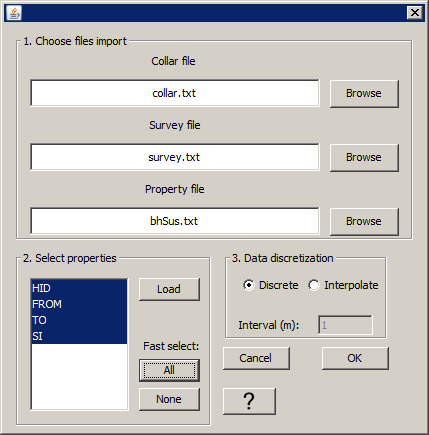
\includegraphics[width=0.8\textwidth]{images/BHSS/BHimport1.PNG}}
    \caption{The first \ac{GUI} for importing bore hole data}
    \label{fig:BHimport1}
\end{figure}

There are two methods to link property and drilling data,  discrete and interpolation. If the discrete option is selected then GIFtools simply determined the spatial location based on the depth provided in the property file. In the case that the depth is given in the form of a ``from'' and a ``to'' depth, the depth of the measurement is considered to be the mean of the two depths. 

If interpolate is selected the program behaves differently if the depth information is simple depths or a ``from'' and a ``to'' depth. In the case of simple depths, it is assumed that the measurement is some physical property, and given the sample distance in the \ac{GUI} the measurements are linearly interpolated along the bore hole. In the case of ``from'' and ``to'' depths it is assumed that the measurement lithologies and depths along the hole that are within a ``from'' and ``to'' interval are assigned the property given while depths outside of any range are assigned a NaN value.






\begin{itemize}
 \item Show \ac{GUI}s to do this.
 \item describe options in importing data
\end{itemize}



\subsection{Visualizing Bore Hole Data}
\label{subsec:visBH}

\subsection{Converting Lithogy Information into Petrophysical Information}
\label{subsec:lithBH}

\subsection{Discretizing Bore Hole Data}
\label{subsec:discBH}

\begin{itemize}
 \item Provide mesh, Usually from Model Builder
 \item describe distribution 
 \begin{itemize}
  \item normal
  \item log normal
  \item describe why one and not other. Cond tends to be log normal (citation needed), Den tends to be normal (citation needed), Susc can be either depending on who you ask(citation needed).
 \end{itemize}
 \item describe method of determining bounds
 \begin{itemize}
  \item Confidence interval: given a number of samples in a cell and a distribution, bounds are determined from a given percent confidence interval. Where the standard deviation is zero, (if there is only one datum, or all the data are equal) he minimum value is used in place of the confidence interval.
  \item Floor: Simply assigns a bound based on the mean value of each cell plus or minus the provided floor value
  \item Standard Deviation: Calculates the standard deviation of the sample values in each mesh cell (given a normal or log normal distribution). The bounds are set as equal to the mean value plus some multiple of the standard deviation. In the case that the standard deviation is zero the minimum value is used instead of the multiplied standard deviation. 
 \end{itemize}
 \item positivity simply set the lower bound and mean to be at least 0
\end{itemize}

\subsection{Editing Bore Hole Data}
\label{subsec:visBH}

\begin{itemize}
 \item show editing of BH discretization
 \item show editing of prop data for susc to eff susc
\end{itemize}

\subsection{Making Constraint}
\label{subsec:makeConstBH}

\begin{itemize}
 \item show resolve conflicts dialogue
 \begin{itemize}
  \item steal from below section (new images necessary)
 \end{itemize}
\end{itemize}

\subsection{Surface Sample}
\label{subsec:SS}

In addition to physical property measurements down hole, physical properties can also be measured on the surface, in many cases with much more ease. As with bore hole data, much work  has been done on including surface sample information in inversion regularization. Surface Samples take on increased importance since in general the sensitivity of the data on a given cell is higher when the cell is nearer the surface. Constraining these surface cells can reduce artifacts that come from this increased sensitivity.

\begin{itemize}
 \item show loading, visualization, editing, all similar to BH
\end{itemize}


\section{Including Geological Maps in Inversion Regularization}
\label{sec:maps}

It is often the case that geological information is provided in the form of geological maps in either cross section or plan view. Such maps are particularly useful since they provide a great deal of information over their entire surface. Cross sections can provide information at depth and constrain a whole region often within the center of a target of interest. Plan view maps do not provide information at depth, but they do constrain the entire surface of the region being inverted.  Constraining the surface of an inversion is of interest since the sensitivity of the data to the top cells is particularly high, which can lead to artifacts on the surface. For the next section the plan view model is from the El Poma case study and the cross section model is from TKC, specifically the map from \citep{harder2006geology}

Below in point form is the method I have developed to incorporate pixel maps.

\subsection{ Preprocessing images}
\label{subsec:Preprocessing images}

Often a geological map image will not be immediately suitable to the methods used below and some prepossessing is required. The most notable features that are undesirable in a map are geological units that are not only one or two colours and text or other annotations that could be interpreted by the program as geological information. Also map images may be of too high resolution to be efficiently used in these methods and must also be down-sampled to save  computer processing time and memory.

 \begin{figure} [h]
    \centering
    \frame{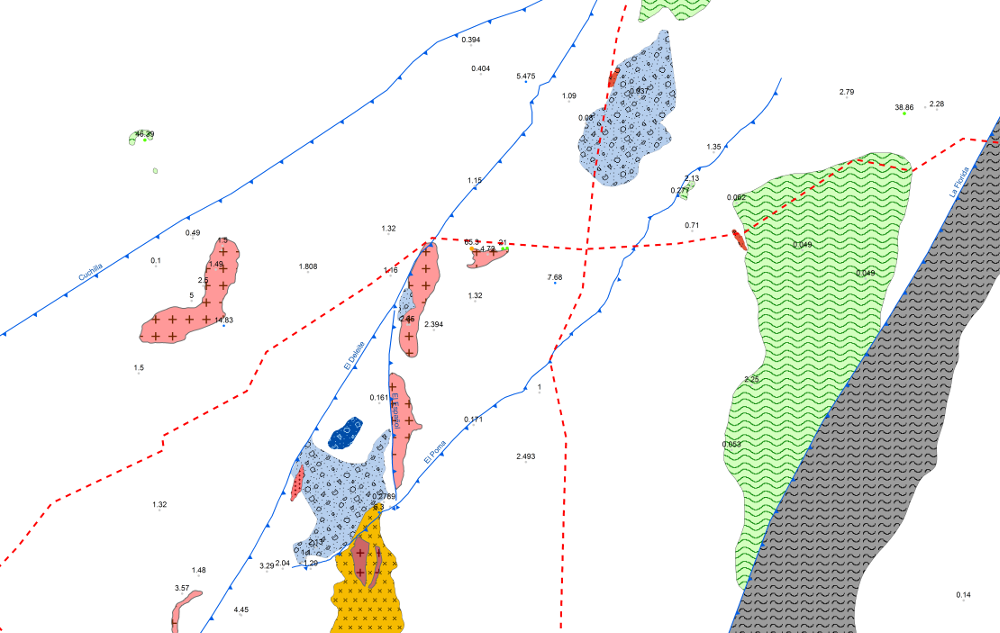
\includegraphics[width=0.8\textwidth]{images/Faults/ElPoma_GEOL_MagSus.png}}
    \caption{The El Poma map with fault lines (blue lines with barbs) included}
    \label{fig:ElPoma_GEOL_MagSus}
\end{figure}

For example \autoref{fig:ElPoma_GEOL_MagSus} has great deal of information, (faults, magnetic susceptibility surface samples, etc.) that are not information about geological units. In addition the geological units are not a single colour polygon. The image has been edited in the GNU Image Manipulation Program (GIMP), a free image editing program, to produce \autoref{fig:ElPoma_GEOL_MagSus_M2M_downsample8}. 

 \begin{figure} [h]
    \centering
    \frame{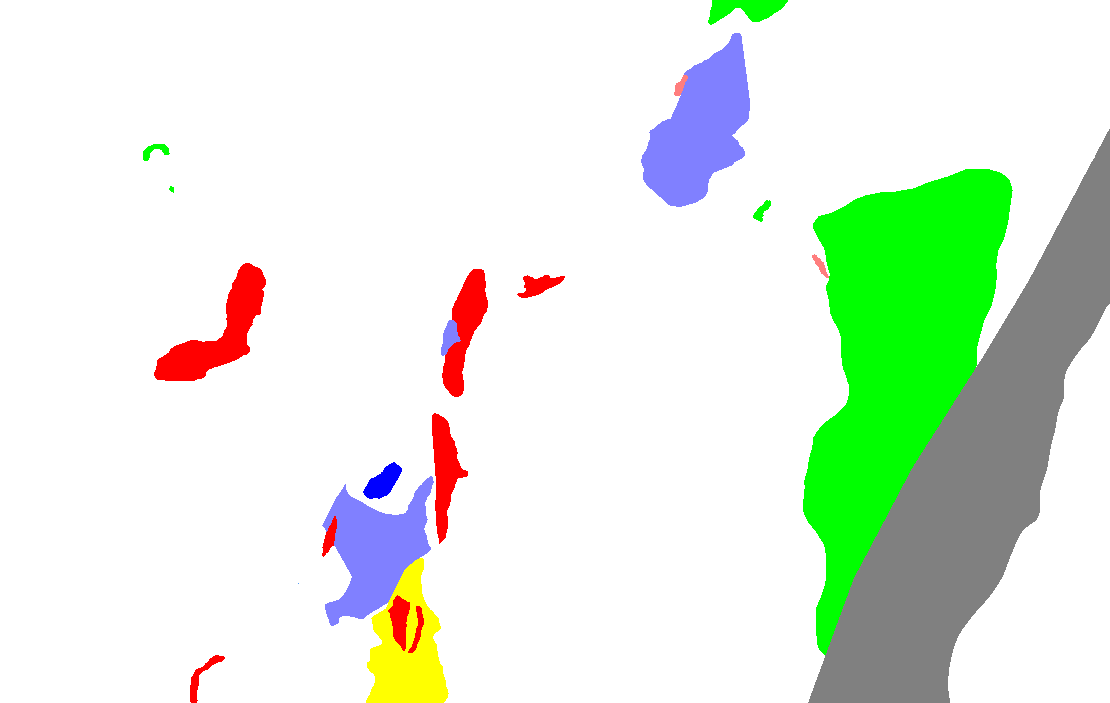
\includegraphics[width=0.8\textwidth]{images/MaptoModel/ElPoma_GEOL_MagSus_M2M_downsample8.png}}
    \caption{The El Poma map with extra information removed and geological units made a single colour}
    \label{fig:ElPoma_GEOL_MagSus_M2M_downsample8}
\end{figure}

\FloatBarrier
\subsection{Loading Images into GIFtools}
\label{subsec:Load Images into GIFtools}

\begin{itemize}
\item load image into the GIFtools format (\autoref{fig:importPlanGui})
\begin{itemize}
	\item Determine image format.
	\item Load image using MATLAB utilities.
	\item Convert image into .png style representation for faster computation.
	\item Using .twf file (world file) assign location and spacial resolution to the image.
	\item Assign a legend linking pixel RGB values to geological unit.
	\item Assign topography (either number or GIFtools TOPOdata item) for visualization.
	\begin{itemize}
		\item In the case of a cross section image, instead of topography, information for the location of the cross section in 3D or 2D space is required (\autoref{fig:importCrossGui}).
	\end{itemize}
\end{itemize}
\end{itemize}
\begin{figure} [h]
    \centering
    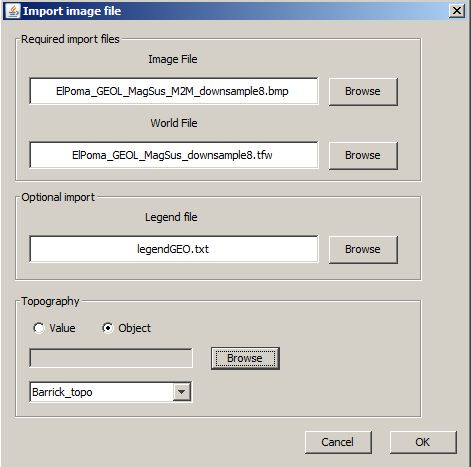
\includegraphics[width=0.5\textwidth]{images/MaptoModel/importPlan.PNG}
    \caption{\ac{GUI} for importing plan view image }
    \label{fig:importPlanGui}
\end{figure}
\begin{figure} [h]
    \centering
    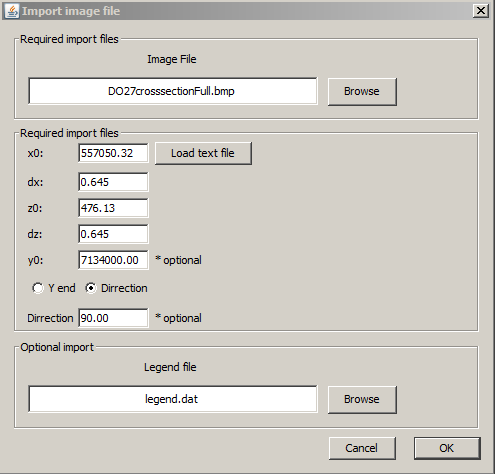
\includegraphics[width=0.5\textwidth]{images/MaptoModel/importCross.PNG}
    \caption{\ac{GUI} for importing cross section image }
    \label{fig:importCrossGui}
\end{figure}
Storing a map as a GIFtools object allows its use in several ways. Notably it allows the integration of the map with models and data, allowing figures overlaying the map and data or model and allowing interpretation of the data or model with direct reference to the map (\autoref{fig:mapData}).
\begin{figure} [h]
    \centering
    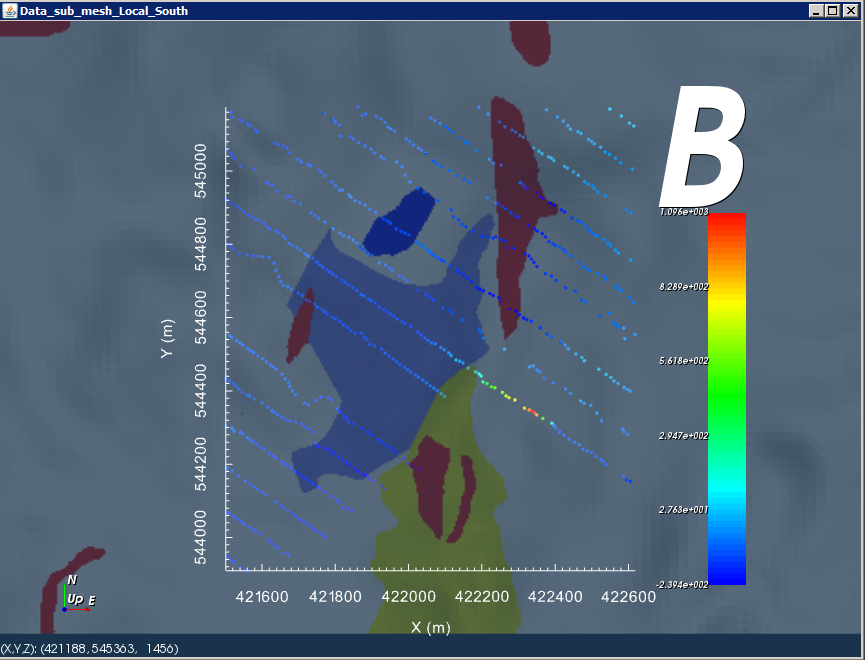
\includegraphics[width=0.5\textwidth]{images/MaptoModel/mapData.PNG}
    \caption{Example of magnetics data being viewed with a map overlaid }
    \label{fig:mapData}
\end{figure}



\subsection{Creating a Pixel Map Legend}
\label{subsec:Create Pixel Map Legend}

Continuing on in the process of making a geological constraint.
\begin{itemize}
\item Find the geological unit represented of each pixel.
\begin{itemize}
	\item In the .png style format as stored in MATLAB, an image consists of an ``image'' field, a matrix of integers, and a ``map'' field, which maps the image matrix to RBG value triplets.
	\item Each RGB triplet is compared to the legend that was provided when the image was loaded. A map field entry is considered to represent a geological unit if all three components of the RGB triplet are within a provided tolerance of any entry in the legend.
	\item Now that we have a relation of entries in the map field to geological units in the legend, we can assign a geological unit to each pixel in the original image simply by applying the new geological map to the image field.
\end{itemize}
\end{itemize}

\subsection{Making a Geology Model from Map}
\label{subsec:Make Geology Model from Map}

\subsubsection{Plan View}
\label{subsubsec:Make Geology Model from Map Plan View}

\begin{itemize}
\item Provide active model. For convenience this is usually an active model already associated with a Model Builder object.
\begin{itemize}
	\item The active model simultaneously provides a discretized topography for the map to lay along and also a mesh (\ac{GIF} 3D tensor or OcTree).
\end{itemize}
\item Provide some form of depth information.
\begin{itemize}
	\item Thickness, a certain amount of depth below topography at each point will be assigned the geological unit at each.
	\item Depth, the map will be used to assign a geological unit down to a fixed depth across the whole model.
	\item Surface, if you provide another surface below topography the cells between topography and the other surface will be assigned.
\end{itemize}

\item Crop all pixels that extend outside of the mesh or that represent the background geological unit.
\begin{itemize}
	\item The cropping greatly speeds up the process and makes it require much less computer memory.
	\item Furthermore, in the event of a mistake with coordinates the process ends almost instantly as there are few pixels to process.
\end{itemize}
\item Finally the geological model is created.
\begin{itemize}
	\item We determine which cell of the mesh each pixel is in, including those cells below each pixel to account for thickness.
	\item Each cell is assigned a geological unit based on the mode of the geological values of each pixel which colours that cell.  In other words, each cell is identified with the geological unit which fills the greatest proportion of the cell.
	\begin{itemize}
	\item The mode is used since each cell will be a particular unit. Since the property being mapped onto each cell by construction must represent a single geological unit, interpolation between the units will not provide the desired result.
	\end{itemize}
	\item The geology definition which will allow the assignment of physical properties to each geological unit. The result is shown in \autoref{fig:mapModelPlan}, the continuous colour bar is not an indication of a continuous model. All model values are integers that represent geological units in the map.
\end{itemize}
\end{itemize}
\begin{figure} [h]
    \centering
    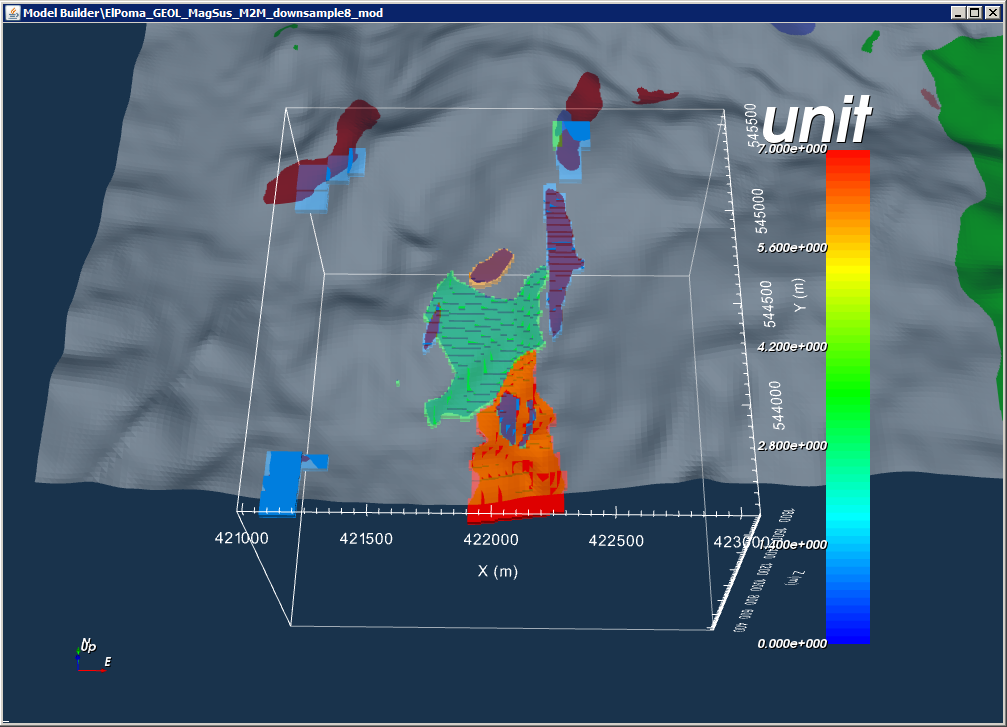
\includegraphics[width=0.5\textwidth]{images/MaptoModel/mapModelPlan.PNG}
    \caption{Example of a geology model created from a map with the map overlaid}
    \label{fig:mapModelPlan}
\end{figure}

\subsubsection{Cross Section}
\label{subsubsec:Make Geology Model from Map Cross Section}

The cross section case follows much the same procedure with a few exceptions. An imported cross section map is shown overlaid on a 2D mesh in \autoref{fig:mapMeshCross}. Notably no parameter for the vertical extent is needed. The other notable exception is that mesh that is used is a \ac{GIF} 2D mesh. The result is shown in \autoref{fig:mapModelCross}.  

A 2D Geology model can be used to create constraints for a 2D inversion, it can also be used to add constraints to a 3D inversion as well. After the 2D geology model is created from the cross section map, it can be inserted into a 3D mesh (\ac{GIF} 3D tensor or OcTree) given a starting and ending position or a starting position and a direction \autoref{fig:add2Dto3D},\autoref{fig:mapModelCross3D}.

\begin{figure} [h]
    \centering
    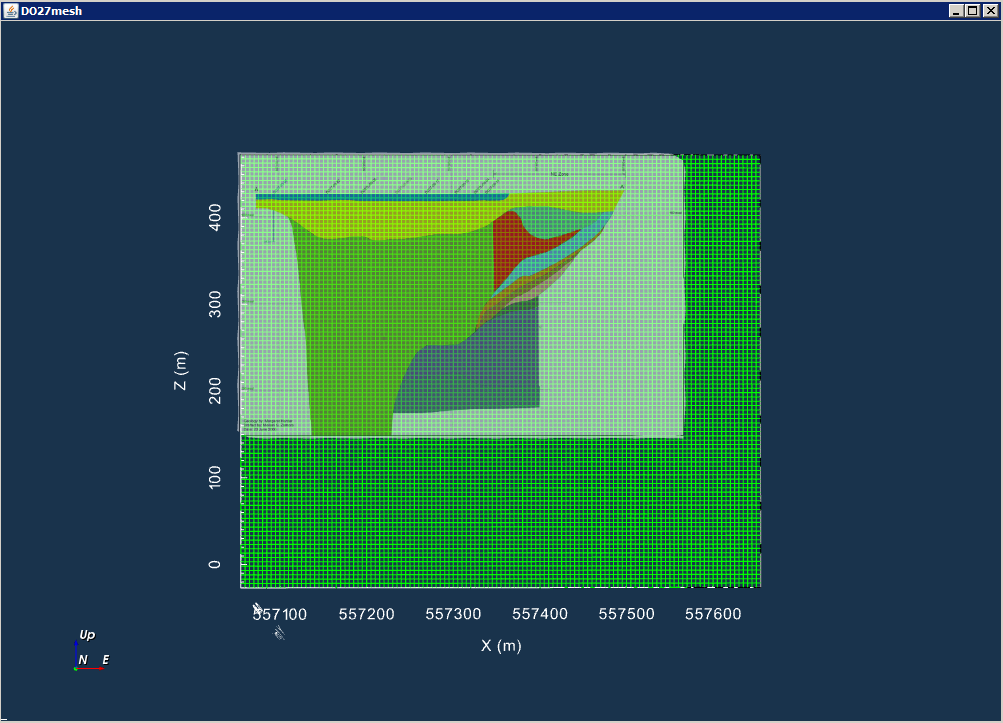
\includegraphics[width=0.5\textwidth]{images/MaptoModel/mapMeshCross.PNG}
    \caption{Example of a 2D mesh with the map overlaid}
    \label{fig:mapMeshCross}
\end{figure}
\begin{figure} [h]
    \centering
    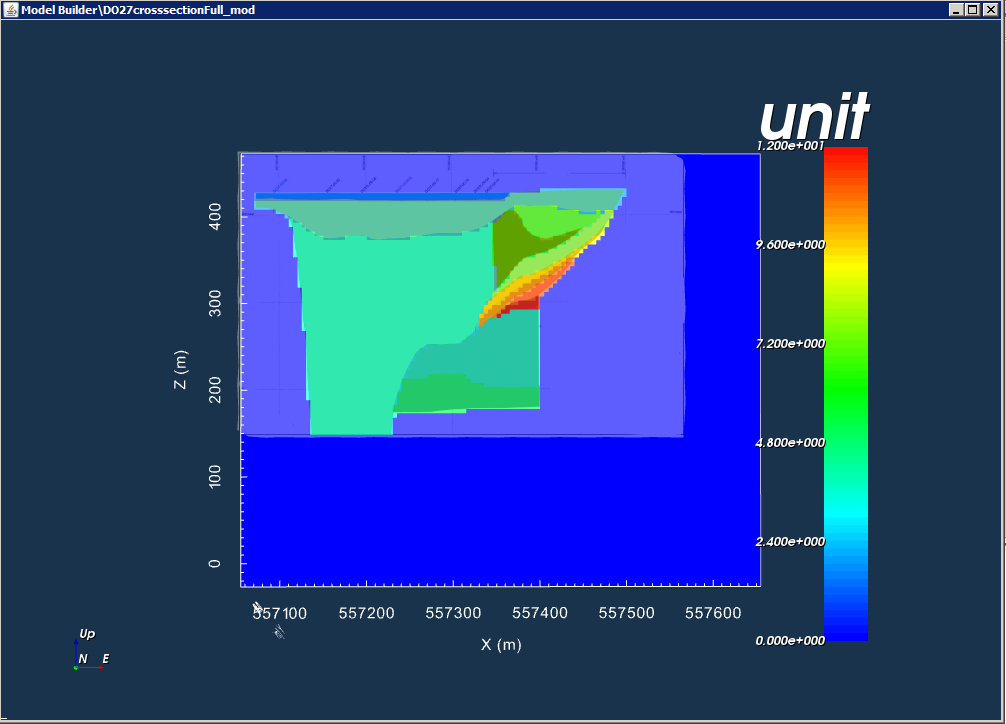
\includegraphics[width=0.5\textwidth]{images/MaptoModel/mapModelCross.PNG}
    \caption{Example of a 2D geology model created from a cross section map with the map overlaid}
    \label{fig:mapModelCross}
\end{figure}
\begin{figure} [h]
    \centering
    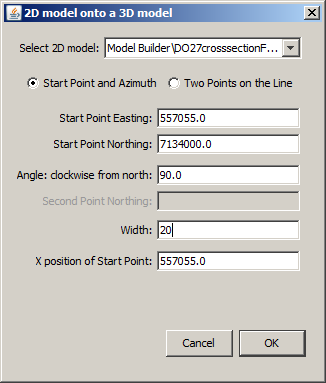
\includegraphics[width=0.5\textwidth]{images/MaptoModel/add2Dto3D.PNG}
    \caption{GUI for adding a 2D model to a 3D model}
    \label{fig:add2Dto3D}
\end{figure}
\begin{figure} [h]
    \centering
    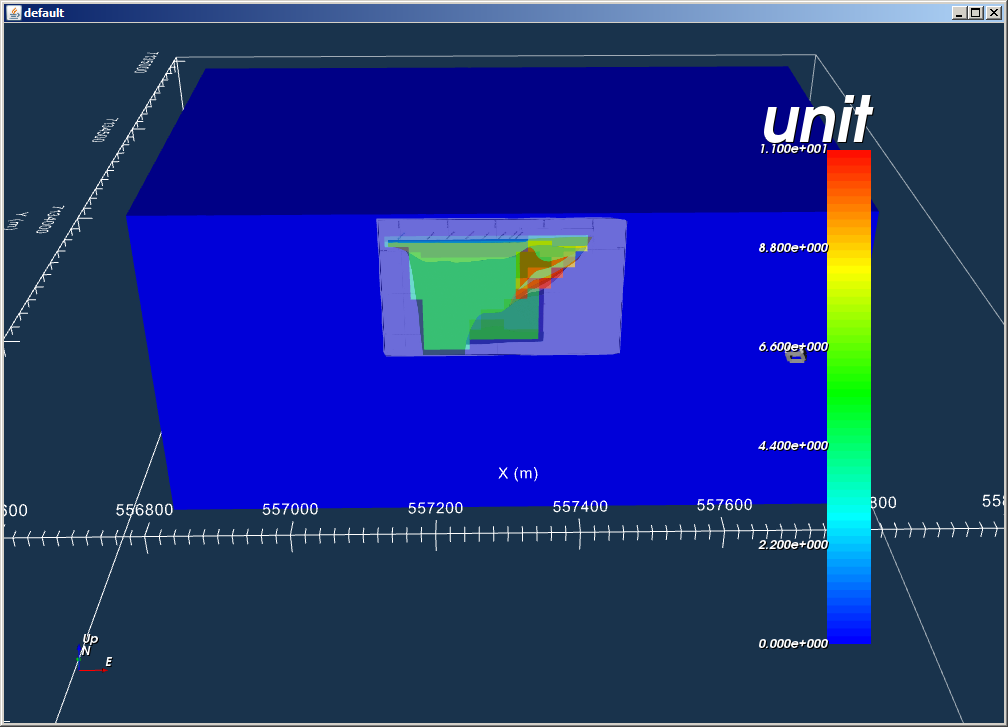
\includegraphics[width=0.5\textwidth]{images/MaptoModel/mapModelCross3D.PNG}
    \caption{Example of a 2D geology inserted into a 3D model with the map overlaid}
    \label{fig:mapModelCross3D}
\end{figure}
\FloatBarrier
\subsection{Making Constraints for an Inversion}
\label{subsec:Making Constraints for an Inversion}

The model that has been created is a geology model. That is, a model in which each cell represents a given geological unit. To be able to convert this model into a constraint for a geophysical inversion the link between between the geology and the petrophysics needs to be provided. 

The link is stored in what is called a geology definition. In GIFtools this takes the form of a lookup table that contains information of each particular geological unit's property, lower and upper bounds, and optionally the smallness weight associated with each unit. 

Using the geology definition we can convert a geology model that has information about the spatial distribution of geological units but not of their physical properties into constraints that are usable by an inversion. In the figures below the geological definition came from surface measurements of magnetic susceptibility within each geological unit. \autoref{fig:geoDefPlan} is an example of a geology definition in the GIFtools GUI.
\begin{figure} [h]
    \centering
    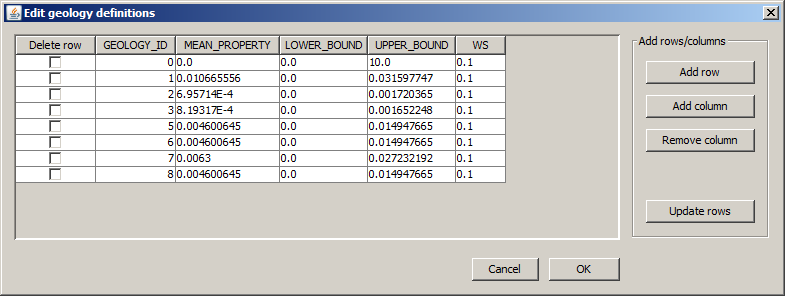
\includegraphics[width=0.8\textwidth]{images/MaptoModel/geoDefPlan.PNG}
    \caption{Example of a geological definition as displayed in the GIFtools GUI}
    \label{fig:geoDefPlan}
\end{figure}

Once the geology definition is provided, we can use the Combine Model Dialog (\autoref{fig:combineModelRef}) in Model Builder to create a reference model and bounds. 
\begin{figure} [h]
    \centering
    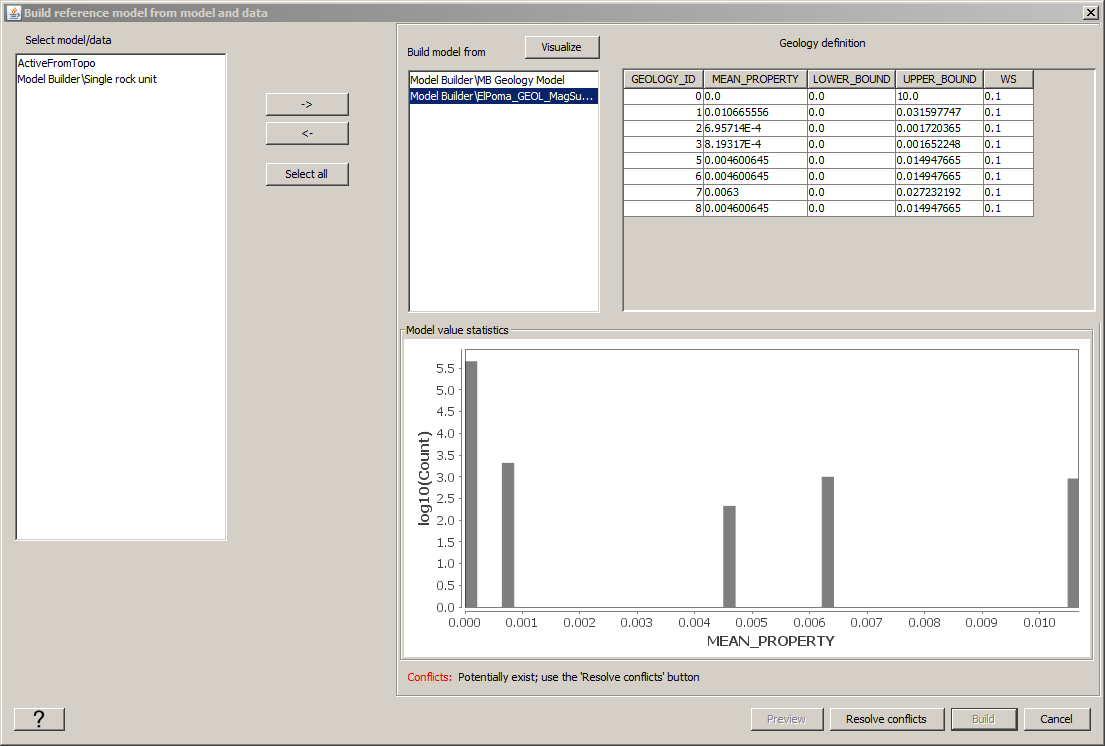
\includegraphics[width=0.8\textwidth]{images/MaptoModel/combineModelRef.PNG}
    \caption{Example of a typical combine model dialog for a reference model}
    \label{fig:combineModelRef}
\end{figure}
In this case the resolution of conflicts is trivial as there is a single source of information. Less trivial examples of the creation of reference models and bounds will be discussed later. The resulting reference model is shown in \autoref{fig:mapRefModPlan}.
\begin{figure} [h]
    \centering
    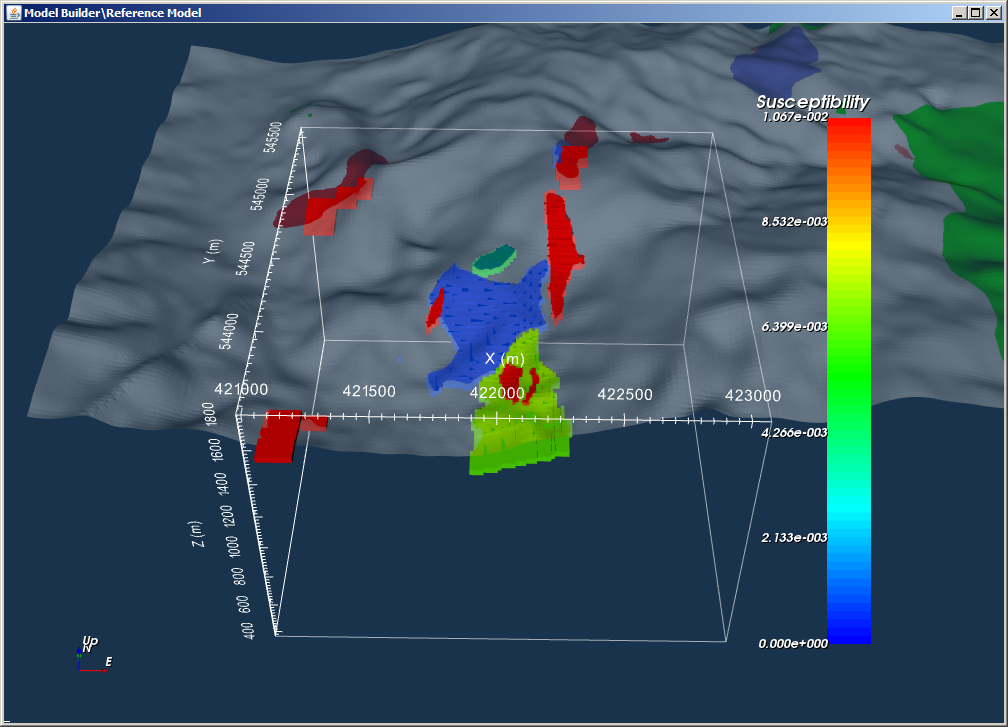
\includegraphics[width=0.8\textwidth]{images/MaptoModel/mapRefModPlan.PNG}
    \caption{Example of a reference model created from a geological map}
    \label{fig:mapRefModPlan}
\end{figure}

\subsection{Inputing Fault information from Geological Maps}
\label{subsec:Inputing Fault information from Geological Maps}

Another piece of information that can be in geological maps are fault locations. Again in the context of El Poma the map provided a whole complex of thrust faults as shown in the un-doctored map in \autoref{fig:ElPoma_GEOL_MagSus}

The method used to insert faults into an inversion is as follows:

\begin{itemize}
\item Determine the end points of the fault.
\begin{itemize}
	\item GIFtools makes this easy by reporting the location of the cursor in the data viewer allowing you to find the location (including elevation) of a point along the fault.
\end{itemize}
\item Using the locations provided create a box of a desired thickness (default value is based on the core mesh size) that includes the ends points of the fault and dips in the desired direction.
\item faces within this box are assigned a new value that is provided in the GUI \autoref{fig:makeFaultGUI}.
\end{itemize}

\begin{figure} [h]
    \centering
    \frame{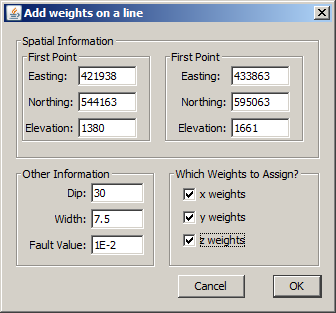
\includegraphics[width=0.5\textwidth]{images/Faults/makeFaultGUI.PNG}}
    \caption{The GUI for the creation of fault weights}
    \label{fig:makeFaultGUI}
\end{figure}

This process can be done multiple times to create non-trivial fault complexes as shown in \autoref{fig:faults}

\begin{figure} [h]
    \centering
    \frame{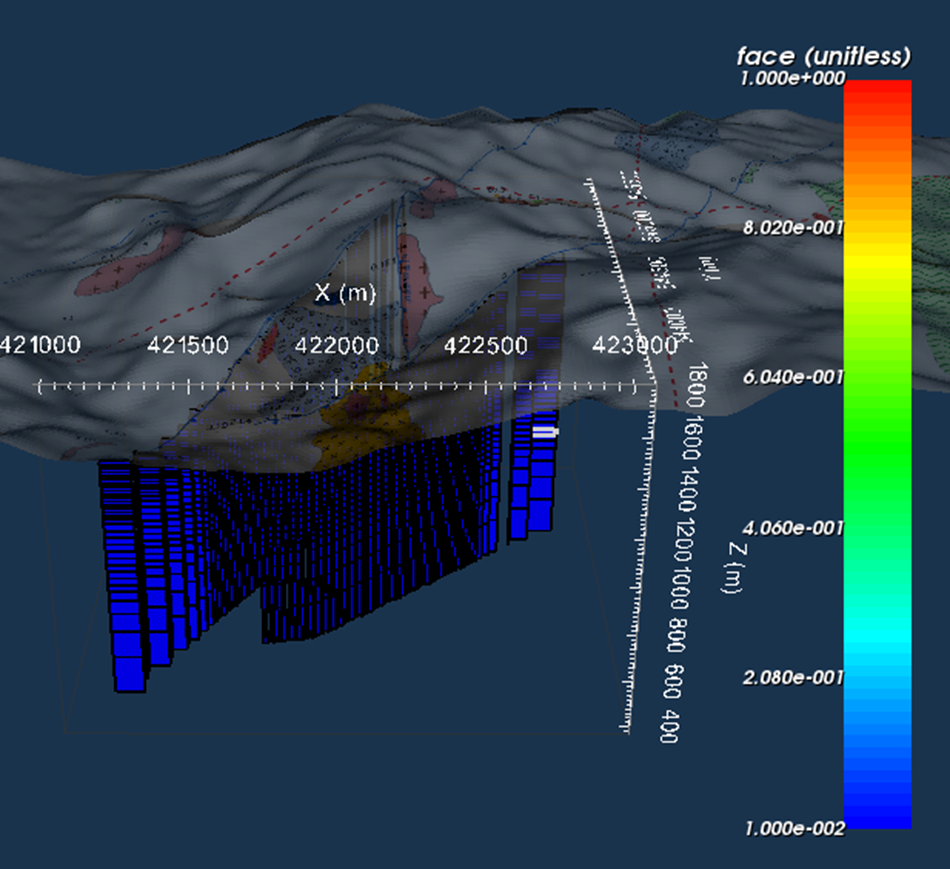
\includegraphics[width=0.5\textwidth]{images/Faults/faults.png}}
    \caption{An example of fault weights that can be created with GIFtools}
    \label{fig:faults}
\end{figure}
\FloatBarrier

\section{Clustering to Create Pseudo-geologic Constraints}
\label{sec:cluster}

\subsection{Clustering Algorithms}
\label{subsec:clusterAlgo}

In contexts where multiple data types have been collected over an area, it is often of interest to include information from one inversion result in the regularization of another. Much work has been done on this topic (see \autoref{sec:Literature Review}).

One possible way of integrating information from another inversion result is through clustering to create pseudo-geological models, and then using these to create reference models, bounds, and smoothness weights to constrain subsequent inversions.

\begin{itemize}
 \item Types of clustering algorithms
 \begin{itemize}
  \item K-mean
  \item C-mean
  \item User Defined bounds
 \end{itemize}
 \item describe algorithm of each
\end{itemize}

\subsection{Clustering In GIFtools}
\label{subsec:clusterTools}

\begin{itemize}
 \item describe requirements
 \item show GUI
 \item show result
\end{itemize}

\subsection{Creation of Constraints}
\label{subsec:clusterConstraints}

\begin{itemize}
 \item show creation of ref and bounds from mean cluster boundaries
 \item show creation of sharp bounds with weights.
\end{itemize}

\section{Voxel-Parametric Inversion to Provide Physical Property Values for Geological Models}
\label{sec:voxelParam}


\begin{itemize}
 \item re-describe forward problem with emphasis on forward operator and the size of the data and model vectors
 \item show that geological model can collapse the forward operator to much smaller matrix by assuming that each unit has a single property value.
 \begin{itemize}
  \item especially when the background is fixed at zeros and has no sensitivity
 \end{itemize}
 \item describe optimization of new parametric inversion with many fewer degrees of freedom
 \item describe uses of the new model
 \begin{itemize}
  \item assign properties to geological models that fit the collected data as closely as possible
  \begin{itemize}
   \item perhaps allows the geology constraints as in \autoref{subsec:clusterConstraints} to be more accurate
   \item allows the determination of magnetization direction given a geologic or pseudo-geologic model of an magnetization anomaly   
   \item allows the creation of synthetic models that roughly fit data that has already been acquired
  \end{itemize}
 \end{itemize}
\end{itemize}



\section{Conclusion}
\label{sec:GIFtoolsConc}

In this section I have shown the creation of constraints that are compatiple with \ac{GIF} inversion codes. I have created these constraints from multiple types of map (Cross Section and Plan View) and have used different pieces of information from these maps (geological units and fault locations).



%\section{Using Multiple Data Types, with Clustering}
%\label{sec:Using Multiple Data Types, with Clustering}
%
%There is interesting things to discuss in the storing of multiple inversion in GIFtools, and in the use of clustering algorythms used and then ability to take geological models and make reference models and non-trivial face weighting.

\endinput

Any text after an \endinput is ignored.
You could put scraps here or things in progress.
